\section{Technical Implementation}
In order to be able to trigger a sonic reaction by the plant by touching it, a reliable sensor with appropriate signal processing needs to be implemented. In this case we chose to measure the capacitance in a way. These changes are picked up by an Arduino, which transfers the data via USB port to a computer. The data is received within a Pure Data patch which decides when to play what kind of samples. In a later attempt we tried a standalone variant with a Raspberry Pi instead of a computer.

\subsection{Measuring Capacitance}
For the capacitance measurement we send a 100 Hz square wave signal through a digital output. This means the binary output switches between 0 and 5 Volts. The signal goes thorugh a $10 M \Omega$ resistor and then into the soil of the plant. The analogue input of the Arduino measures the voltage between the resistor and its internal ground. Since the plant soil is not connected in any way to the internal ground, the voltage between is not defined. A difference in voltage when the resistance changes can be detected nevertheless. 

\begin{figure}[H]
\begin{center}
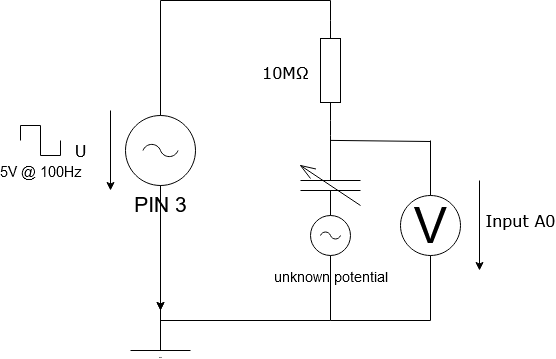
\includegraphics[width=0.7\linewidth]{Figures/schematic1.png}
\caption{Schematic of the measuring set-up}
\end{center}
\end{figure}
Since with this set-up, the measurements change drastically with the environment and used equipment (PC, Raspberry Pi,...) a calibration method was implemented in Pure Data to adjust for the changes.


\subsection{Processing Input Data}
\subsubsection{Arduino}
Once the input data is received, it needs to be filtered. First a DC-Filter is applied since we do not want any DC offsets but also because we do not care for low-frequency content when analysing capacitance. Next, a Root Mean Square value is calculated to smooth out the received data. The input pin is read with a sampling frequency of 800 Hz and every $25^{th}$ sample, a RMS over 1024 samples is sent to the serial output with a alphabetical prefix. Numerical values go from 0 to 1023, the alphabetical prefix determines the sensor (a light sensor or a moistness sensor might be implemented at a later time) so they can be told apart after transmission. 
\subsubsection{Pure Data}
Once the data is received in Pd, it first needs to be converted from ASCII to numbers, so that the algorithm can further process the information:

%\begin{figure}[H]
%\begin{center}
%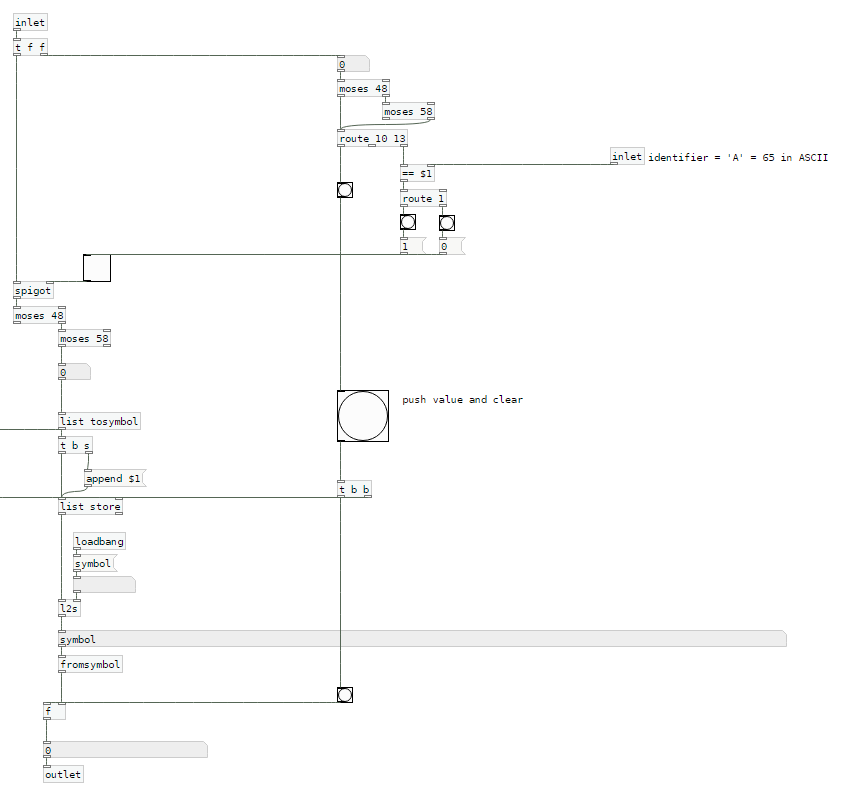
\includegraphics[width=0.7\linewidth]{Figures/ASCII.png}
%\caption{Converting ASCII data received from the Arduino to integers}
%\end{center}
%\end{figure}
Afterwards, the kind of reaction (happy, need or angry) needs to be determined. For this, the program needs to know when a touch occurs. This is achieved by the calibration process. By touching the plant, standing close to it and going away from it during calibration, it sets the thresholds for when it is supposed to detect a touch or proximity.
\begin{itemize}
\item Happy:\\
If the input goes beneath the set threshold, it plays a happy sound (randomly chosen but non repeating). Afterwards the Pd patch ignores all touches for a certain amount of time (as of now 700 miliseconds) before being able to play any sound again. This is necessary because we get about 30 values per second that would trigger 30 sounds within this second if the plant was touched for this entire second.
\item Angry\\
If, within a set amount of time the plant was touched too much, it expresses anger. The amount of time until it becomes annoyed can be set in the GUI. So if, for example, you have been touching it for 4 seconds within the last 10 seconds everything is fine. If you have been holding its leaves for 5 or more seconds in that time it gets angry.
\item Needy
As soon as you let go of the plant, a timer starts counting. If the timer reaches a threshold set in the GUI, the plant becomes needy. This does not mean it constantly makes noises for attention but every second there is a small probability for it to make a noise. If in this state you get in close proximity to the plant (not touching it, just passing by next to it), it will very likely call you out and demand some love.
\end{itemize}

\begin{figure}[H]
\begin{center}
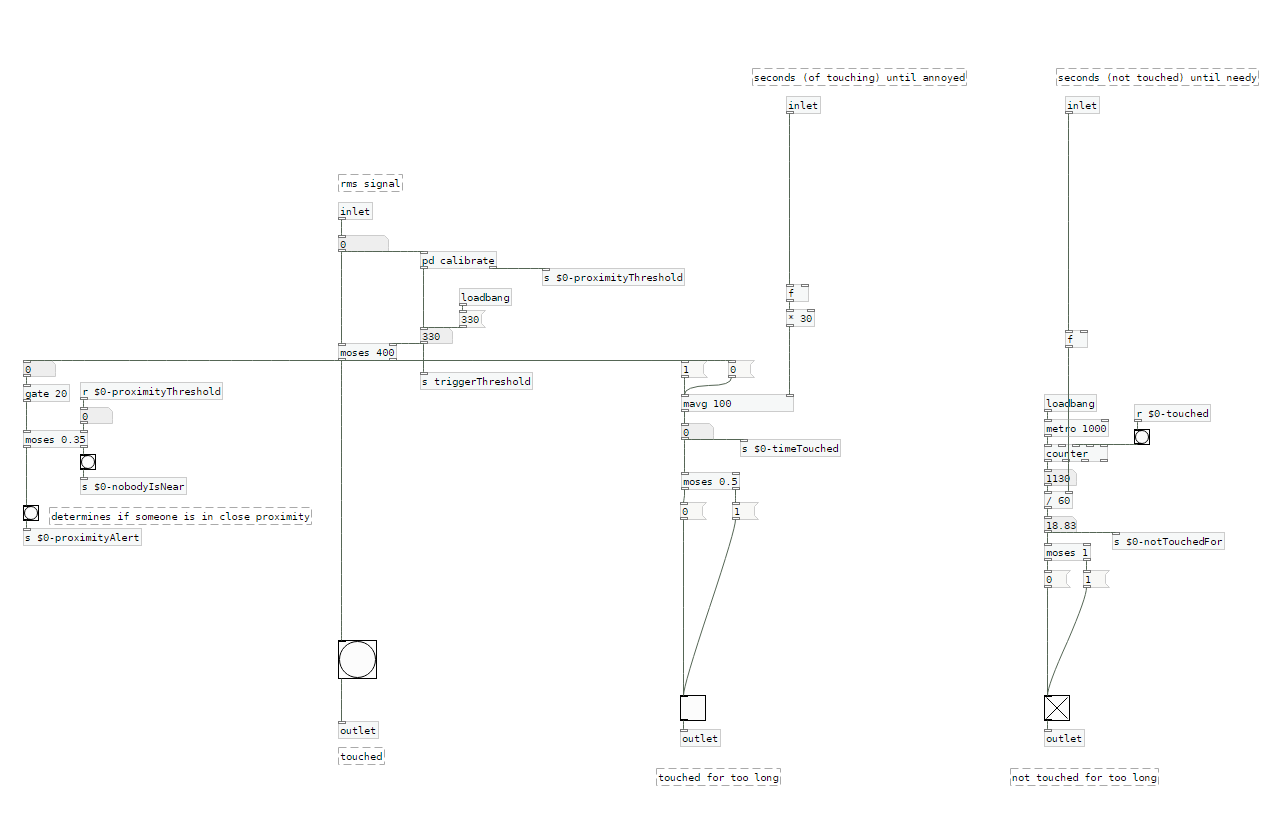
\includegraphics[width=0.9\linewidth]{Figures/calculateTouches.png}
\caption{Calculating if it has been touched, touched for too long or not had any attention for too long}
\end{center}
\end{figure}

\begin{figure}[H]
\begin{center}
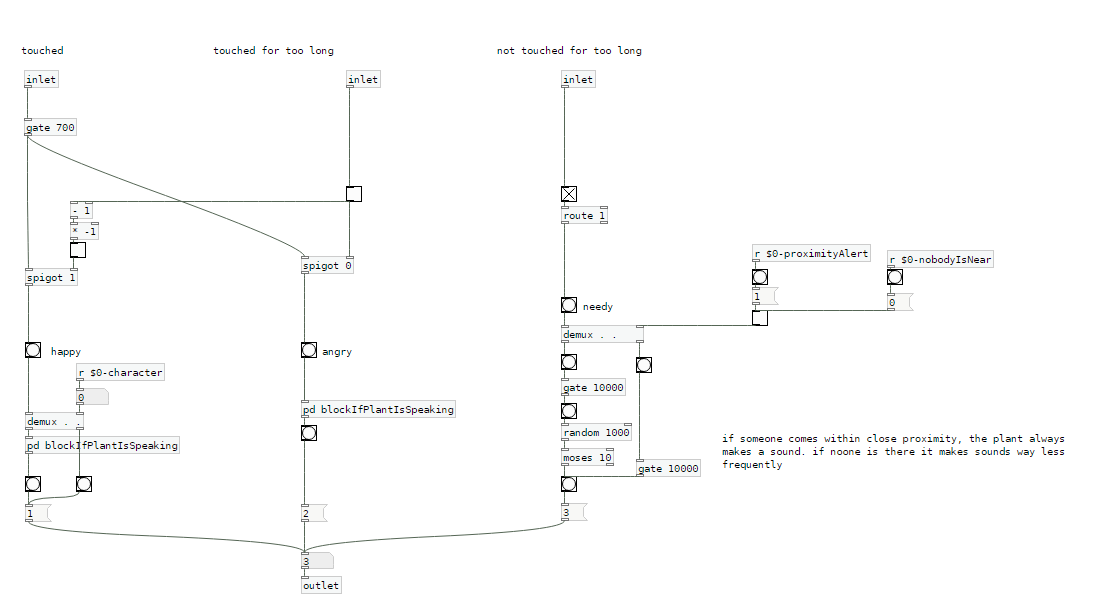
\includegraphics[width=0.9\linewidth]{Figures/decideMood.png}
\caption{Decide on what mood to express}
\end{center}
\end{figure}
\subsubsection{Graphical User Interface}
The GUI in Pd has consists of three parts: Calibration, monitoring and settings.


\begin{figure}[H]
\begin{center}
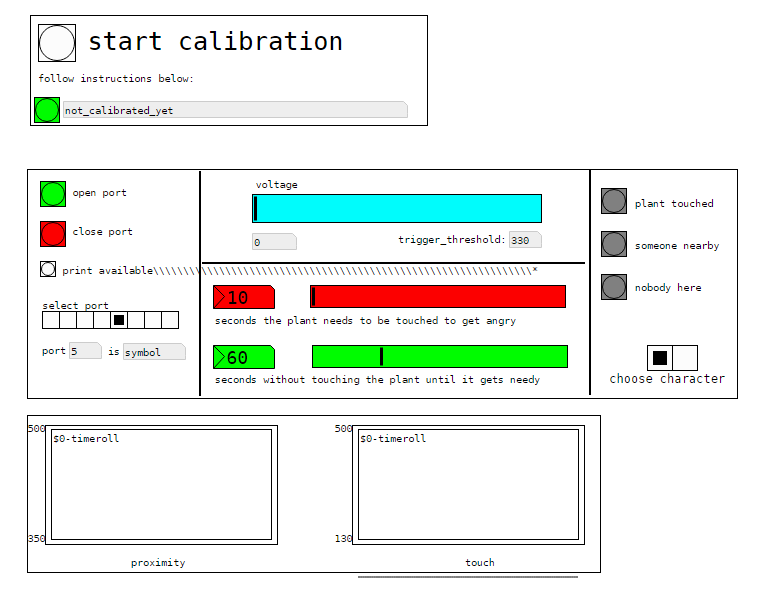
\includegraphics[width=0.9\linewidth]{Figures/GUI.png}
\caption{Graphical User Interface}
\end{center}
\end{figure}


The calibration in the top part has already been described. It sets the correct threshold. Just push the 'start calibration button' and the text field tells you what to do when.
The middle part is mostly for settings like which USD port to read from, opening and closing the port and setting the time for when mood changes occur and what sound character to use (so far we have recorded to different kinds of characters with happy, angry and needy sounds each). Lastly the incoming voltages can be monitored. On the very bottom, two graphical arrays are displayed. If a plant is connected, they show the history of the last 100 samples. The only difference between them is the y-scaling. One is zoomed further in for the proximity detection (visibly only as smaller changes) and one adjusted to the 'touch-threshold'. The buttons on the right display if the algorithm detects a touch, proximity or nothing at all at this very moment. 





\subsection{Standalone Version}
As an additional task, we tried to get the entire system running without needing to connect it to a computer. One reason for this attempt was, that we wanted the project to be a part of an exhibition. Instead of a computer, a Raspberry Pi was used on which Pure Data was installed. Unfortunately the Pd object for reading the serial input did not work. As a workaround a python script was written which reads the serial input and sends the data via OSC, which in turn can be read by Pure Data:
\begin{lstlisting}[style=styC++]
import time
import serial
from pythonosc import udp_client

ser = serial.Serial('/dev/ttyACM0', 9600, timeout=5)
client = udp_client.SimpleUDPClient("127.0.0.1", 8000)
while 1:
    input_string = ser.readline().decode("utf-8").strip()
    print(input_string)
    client.send_message("/A", int(input_string[1:]))
    time.sleep(0.001)
\end{lstlisting}
This script has to be running constantly for the Pd patch to work. If an error occurs (e.g. by unplugging the USB connection shortly), the script may stop and everything will stop working. Additionally, the USB port is set in the script and if the Arduino is plugged in another port it will not work either unless you change the code.
\begin{figure}[H]
\begin{center}
\includegraphics[width=0.75\linewidth]{Figures/setup.jpg}
\caption{Arduino, Raspberry Pi and battery powered speaker}
\end{center}
\end{figure}




